% Source: Code/FLIR_Python/architecture_diagrams/tracking_process_architecture.tex
\documentclass[border=10pt]{standalone}
\usepackage{tikz}
\usepackage{xcolor}
\usetikzlibrary{shapes.geometric, arrows.meta, positioning, fit, backgrounds, calc}

% USC Color Definitions
\definecolor{uscgarnet}{HTML}{73000a}
\definecolor{uscatlantic}{HTML}{466A9F}
\definecolor{usccongaree}{HTML}{1F414D}
\definecolor{uschorseshoe}{HTML}{65780B}
\definecolor{uscrose}{HTML}{CC2E40}
\definecolor{uscsandstorm}{HTML}{FFF2E3}
\definecolor{uscwarmgrey}{HTML}{676156}

\begin{document}

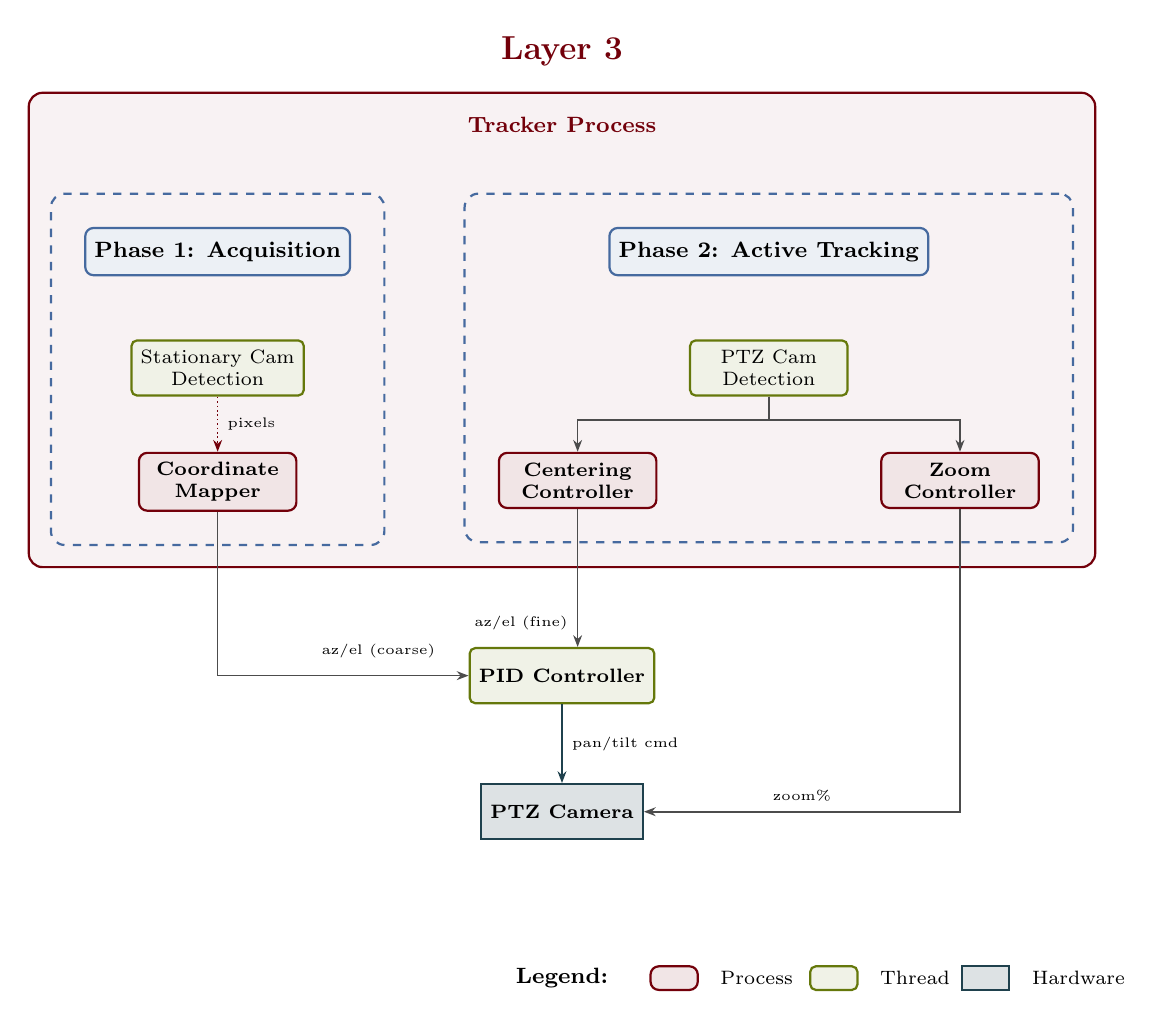
\begin{tikzpicture}[
    % Node styles (USC Colors)
    input/.style={rectangle, draw=uschorseshoe, fill=uschorseshoe!10, thick, minimum width=2cm, minimum height=0.7cm, align=center, rounded corners=2pt, font=\scriptsize},
    process/.style={rectangle, draw=uscgarnet, fill=uscgarnet!10, thick, minimum width=2cm, minimum height=0.7cm, align=center, rounded corners=3pt, font=\scriptsize\bfseries},
    controller/.style={rectangle, draw=uschorseshoe, fill=uschorseshoe!10, thick, minimum width=1.8cm, minimum height=0.7cm, align=center, rounded corners=2pt, font=\scriptsize\bfseries},
    output/.style={rectangle, draw=usccongaree, fill=usccongaree!15, thick, minimum width=2cm, minimum height=0.7cm, align=center, font=\scriptsize\bfseries},
    phase/.style={rectangle, draw=uscatlantic, fill=uscatlantic!10, thick, minimum width=3cm, minimum height=0.6cm, align=center, rounded corners=3pt, font=\footnotesize\bfseries},
    trackerbox/.style={draw=uscgarnet, thick, rounded corners=5pt, inner sep=15pt},
    container/.style={draw=uscatlantic, thick, dashed, rounded corners=5pt, inner sep=12pt},
    % Arrow styles
    dataarrow/.style={-{Stealth[length=1.5mm]}, semithick, draw=black!70},
    ipc/.style={-{Stealth[length=1.5mm]}, semithick, draw=uscgarnet, densely dotted},
    http/.style={-{Stealth[length=1.5mm]}, semithick, draw=usccongaree},
]

% Top alignment coordinate
\coordinate (topcenter) at (0,0);

% ============================================================================
% PHASE 1: ACQUISITION (Left side)
% ============================================================================
\node[phase, below=2cm of topcenter, xshift=-3.5cm] (phase1) {Phase 1: Acquisition};

% Stationary camera input (external reference)
\node[input, below=0.8cm of phase1] (statcam) {Stationary Cam\\Detection};

% Coordinate converter
\node[process, below=0.7cm of statcam] (coord) {Coordinate\\Mapper};

% Phase 1 box will be drawn later after tracker process

% Phase 1 connections
\draw[ipc] (statcam) -- node[right, font=\tiny] {pixels} (coord);

% ============================================================================
% PHASE 2: ACTIVE TRACKING (Right side)
% ============================================================================
\node[phase, below=2cm of topcenter, xshift=3.5cm] (phase2) {Phase 2: Active Tracking};

% PTZ camera detection input
\node[input, below=0.8cm of phase2] (ptzcam) {PTZ Cam\\Detection};

% Centering controller - positioned to the left
\node[process, below left=0.7cm and 0.4cm of ptzcam] (center) {Centering\\Controller};

% Zoom controller - positioned to the right
\node[process, below right=0.7cm and 0.4cm of ptzcam] (zoom) {Zoom\\Controller};

% Phase 2 box will be drawn later after tracker process

% Phase 2 connections
% Phase 2 connections - ortho connections to split flows
\draw[dataarrow] (ptzcam.south) -- ++(0,-0.3) -| (center.north);
\draw[dataarrow] (ptzcam.south) -- ++(0,-0.3) -| (zoom.north);

% ============================================================================
% TRACKER PROCESS BOX - wrapping both phases with label inside (draw first)
% ============================================================================
% Helper coordinate to make box taller at top
\coordinate (trackertop) at ($(topcenter) + (0,-1.0)$);

\begin{scope}[on background layer]
    \node[trackerbox, fill=uscgarnet!5, fit=(trackertop)(phase1)(statcam)(coord)(phase2)(ptzcam)(center)(zoom), inner sep=20pt] (trackerprocess) {};
\end{scope}
% Tracker Process label inside the box at top
\node[font=\footnotesize\bfseries, uscgarnet, anchor=north] at ([yshift=-0.2cm]trackerprocess.north) {Tracker Process};

% Title - centered on the tracker process box
\node[font=\bfseries\large, uscgarnet, anchor=south] (title) at ([yshift=0.2cm]trackerprocess.north) {Layer 3};

% Now draw phase containers ON TOP of tracker process
\node[container, fill=none, fit=(phase1)(statcam)(coord)] (p1box) {};
\node[container, fill=none, fit=(phase2)(ptzcam)(center)(zoom)] (p2box) {};

% ============================================================================
% PID CONTROLLER (Thread - outside process, inside layer)
% ============================================================================
\node[controller, below=1cm of trackerprocess] (pid) {PID Controller};

% ============================================================================
% PTZ CAMERA (Hardware - outside layer)
% ============================================================================
\node[output, below=1cm of pid] (ptz) {PTZ Camera};

% ============================================================================
% CONNECTIONS BETWEEN PHASES AND SHARED COMPONENTS
% ============================================================================

% Phase 1 → PID (coarse positioning) - go down, then right angle to pid.west
\draw[dataarrow] (coord.south) |- (pid.west);
\node[above left=0.1cm and 0.3cm of pid.west, font=\tiny] {az/el (coarse)};

% Phase 2 → PID (fine tracking) - straight down to PID top
\draw[dataarrow] (center.south) -- (center |- pid.north) node[above left, font=\tiny, pos=0.95] {az/el (fine)};

% Zoom → PTZ (direct zoom control) - go down then right angle to ptz.east
\draw[dataarrow] (zoom.south) |- node[above, font=\tiny, pos=0.75] {zoom\%} (ptz.east);

% PID → PTZ
\draw[http] (pid) -- node[right, font=\tiny] {pan/tilt cmd} (ptz);

% ============================================================================
% Legend
% ============================================================================
\node[below=1.5cm of ptz, font=\footnotesize\bfseries] (legend) {Legend:};

\node[process, right=0.4cm of legend, minimum width=0.6cm, minimum height=0.3cm] (lp) {};
\node[right=0.15cm of lp, font=\scriptsize] {Process};

\node[controller, right=0.8cm of lp, minimum width=0.6cm, minimum height=0.3cm, xshift=0.6cm] (lt) {};
\node[right=0.15cm of lt, font=\scriptsize] {Thread};

\node[output, right=0.8cm of lt, minimum width=0.6cm, minimum height=0.3cm, xshift=0.5cm] (lh) {};
\node[right=0.15cm of lh, font=\scriptsize] {Hardware};

\end{tikzpicture}

\end{document}
